\section{Artigo Correlato}

% ----------------------------------------------------------------------------------------------------------
\begin{frame}{Artigo Correlato}
Utiliza MCDA para analisar a vulnerabilidade das meso-regiões de Minas Gerais, contribuindo para o direcionamento de políticas públicas;

\begin{columns}

\column{0.55\textwidth}
	
	\begin{block}{Vulnerabilidade}
	Grau de exposição à doença por um conjunto de aspectos individuais ou coletivos;
	\end{block}
	
	\begin{block}{Conjuntos de Critérios}
	Sociais, demográficos, econômicos, infraestrutura de saúde, população em risco e epidemiológicos;
	\end{block}
	
\column{0.45\textwidth}
	\begin{figure}[!h]  
		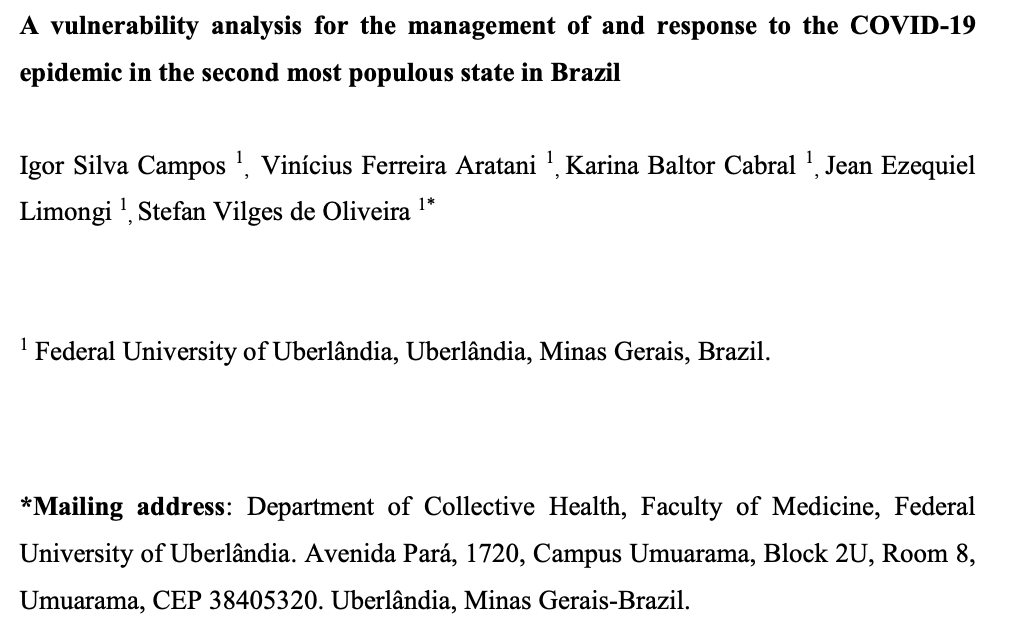
\includegraphics[width=\textwidth]{figs/artigo}
	    \label{fig:artigo}
\end{figure}

\end{columns}
	
\end{frame}
% ----------------------------------------------------------------------------------------------------------
\begin{frame}{Artigo Correlato}

\begin{columns}


\column{0.4\textwidth}
	
	\begin{figure}[!h]  
		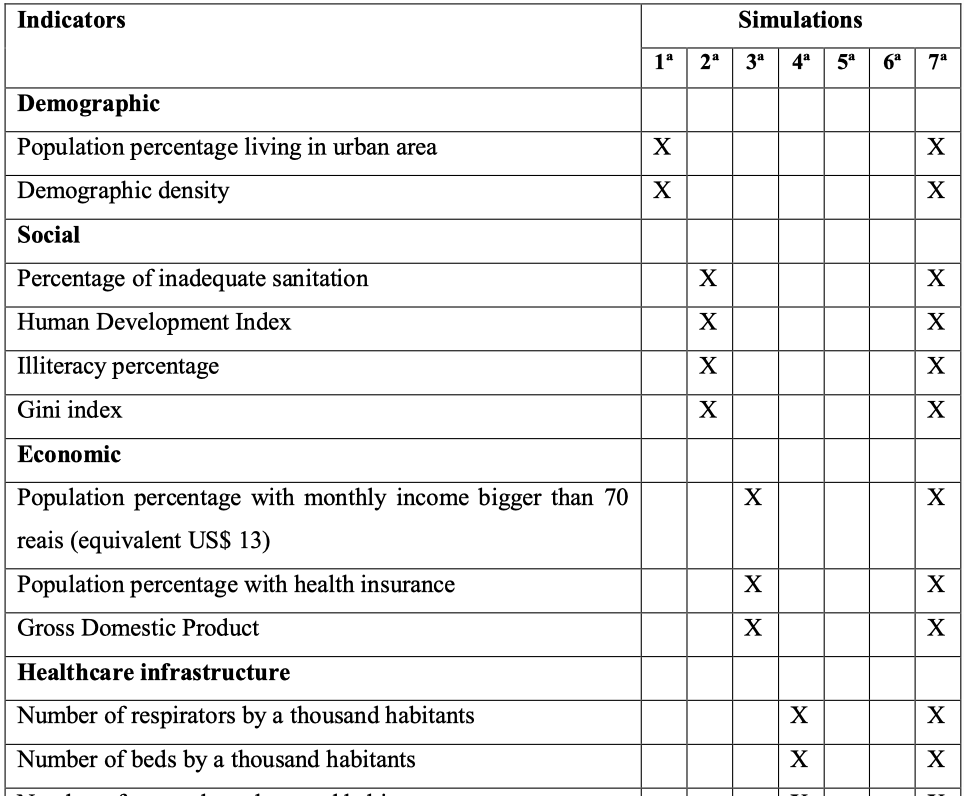
\includegraphics[width=\textwidth]{figs/artigo-simulations}
	    \label{fig:artigo-simulations}
	\end{figure}
	
\column{0.6\textwidth}

\begin{block}{Recursos}
\begin{itemize}
	\item	\textbf{PROMETHEE} - Preference Ranking Method for Enrichment Evaluation\\
	\item \textbf{PRADIN} - Programa de Apoio à Tomada de Decisão baseado em Indicadores
\end{itemize}
\end{block}

\begin{block}{Simulações Realizadas}
\begin{itemize}
	\item 6 Simulações com conjuntos diferentes
	\item 1 Simulação com todos os conjuntos
\end{itemize}	
\end{block}

\end{columns}

Resultados foram interpretados como uma escala de vulnerabilidade, com notas de 1 a 5 para cada meso-região.

\end{frame}
% ----------------------------------------------------------------------------------------------------------
\begin{frame}{Artigo Correlato}

\begin{columns}

\column{0.65\textwidth}

	\begin{figure}[!h]  
		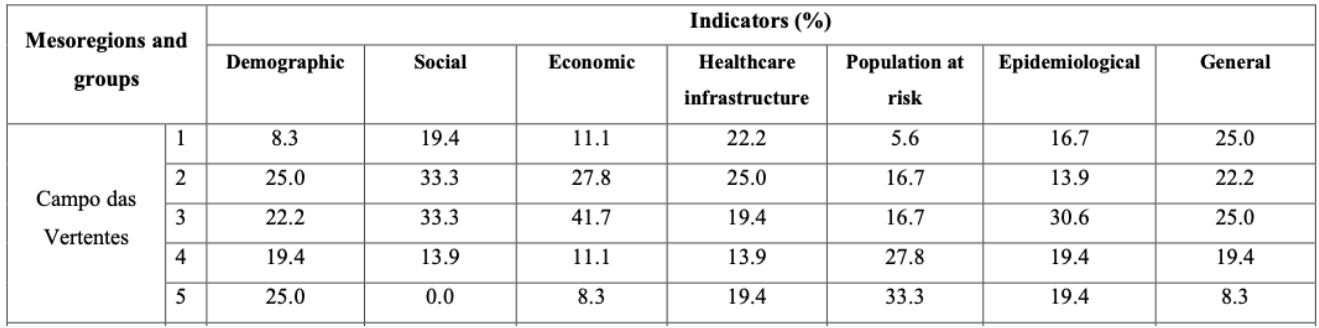
\includegraphics[width=\textwidth]{figs/artigo-results}
	    \label{fig:artigo-results}
	\end{figure}
	
	\begin{itemize}
		\item Estudo realizado para cada município do estado;
		\item Tabela agrupa os municípios por meso-região e indica a porcentagem de municípios em cada grau de vulnerabilidade;
		\item Maior vulnerabilidade em regiões urbanas, devido as características da COVID-19.
	\end{itemize}

\column{0.3\textwidth}
	
	\begin{figure}[!h]  
		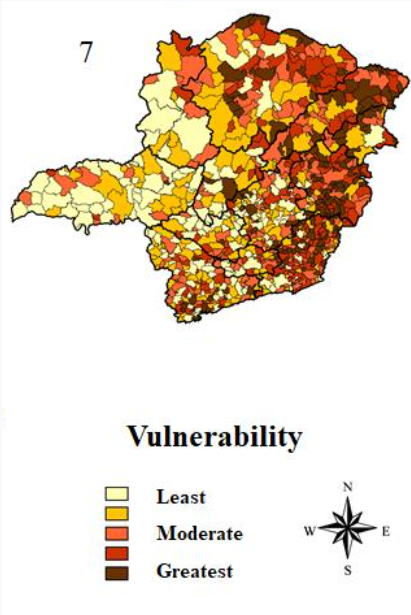
\includegraphics[width=\textwidth]{figs/artigo-vulnerability}
	    \label{fig:artigo-simulations}
	\end{figure}

\end{columns}
\end{frame}

